% !TEX encoding   = UTF8
% !TEX spellcheck = ru_RU
% !TEX root = ../seminars.tex

%%===============================================
\chapter{Графические пользовательские интерфейсы}
%%===============================================

%%====================================
\section{Окно с кнопкой \texttt{Quit}}
%%====================================
Выполним упражнение~1 из~\textbookref{главы~16} учебника. Для~этого пронаследуем \code{My\_window} от~класса \code{Simple\_window} из~библиотеки \code{Graph\_lib}. Затем добавим по~аналогии с~кнопкой \code{Next} кнопку \code{Quit}, как показано на~рисунке~\ref{fig:mywindow}.

\begin{figure}[ht]
    {\centering
        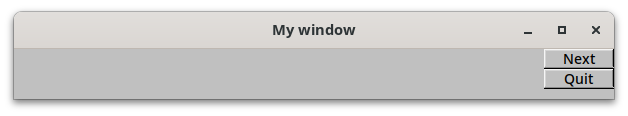
\includegraphics[width=0.6\textwidth]{images/my_window.png}

    }
    \caption{Простое окно \code{My\_window} с кнопкой \code{Quit}}
    \label{fig:mywindow}
\end{figure}

Из~документации к~библиотеке \name{FLTK} известно, что если все окна становятся скрытыми, то цикл обработки событий прекращает работу. То есть для~реализации функции \code{quit()} можно воспользоваться методом \code{hide()}.

\cppfile[firstline=11, lastline=21]{projects/ch16/chessboard/board.h}

Конструктор нашего окна принимает те же аргументы, что и \code{Simple\_window}. Мы добавляем инициализацию кнопки \code{Quit}. Нужно сместить её вниз на~высоту кнопки \code{Next}, которую добавляет базовый класс, а также связать её с~функцией-обработчиком \code{cb\_quit()}:

\cppfile[firstline=7, lastline=12]{projects/ch16/chessboard/board.cpp}

\textbf{NB!} Обратим внимание на одну деталь, которую нам пришлось изменить в~изначальной версии кода библиотеки \code{Graph\_lib}:

\cppfile[firstline=8, lastline=14]{projects/lib/Graph_lib/GUI.cpp}

\noindent В~строке~12 мы передаём указатель на~текущий объект класса (\code{this}), то есть указатель на~кнопку (\code{Button}), а не~указатель на~окно, как это ожидается в~примерах обработчиков, показаных в~\textbookref{главе~16} учебника.

Отметим, что здесь мы можем передавать, вообще говоря, любые данные. Позже библиотека \name{FLTK} вернёт нам указатель на~эти данные в~функцию обратного вызова:

\cppfile[firstline=14, lastline=18]{projects/ch16/chessboard/board.cpp}

\noindent Параметр \code{widget} как раз и есть тот самый адрес кнопки, который мы передаём при~вызове функции \code{Button::attach()}, когда связываем кнопку с~окном:

\cppfile[firstline=11, lastline=11]{projects/ch16/chessboard/board.cpp}

Оказывается, во многих задачах удобнее иметь указатель на~наш виджет. А, так как он хранит адрес окна, с~которым связан, мы можем получить доступ к~нашему окну и, в~конце концов, вызвать метод \code{quit()}:

\cppfile[firstline=17, lastline=17]{projects/ch16/chessboard/board.cpp}

\noindent Здесь использован оператор \code{dynamic\_cast}, который выполняет приведение типа от~ссылки на~объект базового класса к~ссылке на~объект производного класса (\textenglish{down cast}). Такое преобразование в~общем случае небезопасно. Данный оператор выполняет проверку во~время выполнения программы и возбуждает исключение \code{std::bad\_cast} в~случае ошибки.



%%=======================
\section{Шахматная доска}
%%=======================
Покажем, как можно создать клеточное поле и взаимодействовать с~ним на~примере упражнения~2 из~\textbookref{главы~16}. Эти идеи можно использовать для~создания практически любой игры с~клеточным полем: шашек, шахмат, сапёра, морского боя, пять в ряд и других.

Учитывая последующую доработку, код удобно сразу распределить между~несколькими файлами, как это предлагается в~таблице~\ref{tab:chessboard}.

\begin{table}[ht]
    {\centering\begin{tabular}{ll}
        \toprule
        \code{board.h}   & класс \code{Chessboard} для~шахматной доски, а также \code{My\_window} \\
        \code{board.cpp} & \\[0.5em]

        \code{cell.h}    & класс \code{Cell} для~шахматной клетки \\
        \code{cell.cpp}  & \\[0.5em]

        \code{main.cpp}  & \\
        \bottomrule
    \end{tabular}

    }
    \medskip
    \caption{Распределение кода <<шахматной доски>> между файлами}
    \label{tab:chessboard}
\end{table}

Размеры клеток и, соответственно, окна зафиксируем. Впоследствии, такое поведение можно изменить. Клетки представим квадратными кнопками и будем хранить их в~\code{Vector\_ref}. Метки строк и столбцов доски можно нарисовать при~помощи объектов \code{Marks}. Окно, согласно заданию, пронаследуем от~\code{My\_window} из~предыдущего упражнения.

\begin{figure}[ht]
    {\centering
        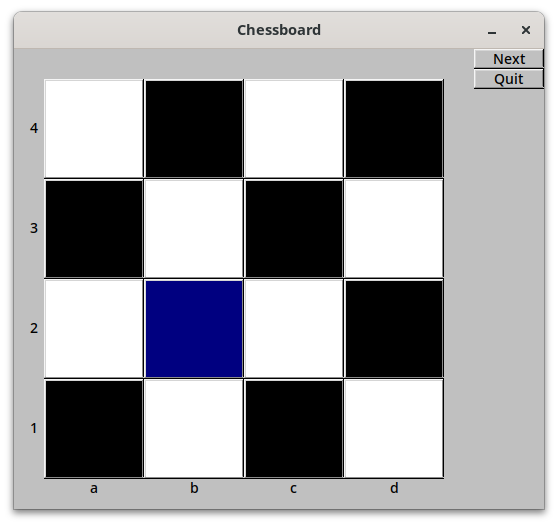
\includegraphics[width=0.5\textwidth]{images/chessboard.png}

    }
    \caption{Окно с шахматной доской \(4\times 4\)}
    \label{fig:chessboard}
\end{figure}

Итак, давайте разбираться по~порядку.



%%===========================
\paragraph{Шахматная клетка.}
%%===========================
Прежде всего, создадим шахматную клетку "--- класс \code{Cell}. Клетки на~шахматной доске могут быть только белыми или чёрными. Это свойство мы выразим, используя перечисление \code{Cell::Type}. Размер клетки зафиксируем на~этапе компиляции. Тогда разумно сделать его константой класса (\code{static}), чтобы обращаться из~любой точки программы без~указания объекта \code{Cell::size}.

Нам придётся перекрыть метод \code{attach()}. Почему?

Также добавим пару методов \code{activate()}/\code{deactivate()} для~управления подсветкой активной клетки (клетка~\code{b2} на~рисунке~\ref{fig:chessboard}), то есть той клетки, которую выбрал мышкой пользователь.

В~заголовочном файле \code{cell.h} разместим определение класса:

\cppfile[firstline=8, lastline=32]{projects/ch16/chessboard/cell.h}

Реализация методов проста и не~требует дополнительных пояснений, кроме того, что \code{pw} "--- это защищённый член класса \code{Graph\_lib::Widget}, связанный с~реальным графическим виджетом из~\name{FLTK}.

Код разместим в~файле \code{cell.cpp}:

\cppfile[firstline=5, lastline=32]{projects/ch16/chessboard/cell.cpp}



%%==========================
\paragraph{Шахматная доска.}
%%==========================
Основные моменты обозначены выше. Отметим здесь, что размер доски (\(N\times N\)) фиксируем на~этапе компиляции. Введём дополнительную константу \(N_{max}\), чтобы пользователь класса не~превышал определённый размер. Дело в~том, что позже мы будем добавлять подписи клеток и пока рассчитываем дизайн максимально на~8--9 клеток по~высоте. Дальше придётся что-то придумывать или каким-то образом выравнивать текстовые метки, состоящие из~двух цифр. (Это оставляем на~подумать.)

В~заголовочный файл \code{board.h} добавим определение класса:

\cppfile[firstline=23, lastline=51]{projects/ch16/chessboard/board.h}

Реализацию методов класса добавим в~файл \code{board.cpp}.

Конструктор задаёт размеры окна, создаёт клетки, располагая их в~соответствующих позициях, и рисует метки строк и столбцов доски. Зафиксируем размеры окна, чтобы пользователь не~смог его растягивать или сжимать. Сделать это позволяет функция \code{size\_range()} "--- метод окна \name{FLTK}.

\cppfile[firstline=48, lastline=67]{projects/ch16/chessboard/board.cpp}
\cpp/  .../
\cppfile[firstline=79, lastline=79]{projects/ch16/chessboard/board.cpp}

Цвет клетки (или тип) вычисляется на~основе номеров строки и столбца, определяющих её положение на~доске. Клетка в~левом нижнем углу имеет чёрный цвет. Обратим внимание, что клетки добавлялись в~линейный массив по~порядку в~соответствии с~направлением снизу вверх и слева направо, как принято в~шахматах.

\cppfile[firstline=20, lastline=26]{projects/ch16/chessboard/board.cpp}



%%=========================
\paragraph{Подписи клеток.}
%%=========================
Метки \code{Marks} допускают всего лишь один символ, поэтому мы используем ограничение \code{N\_max} для~максимального размера доски. Если потребуется вывести двузначные номера клеток, придётся разработать новый класс или добавить метки при~помощи неименованных объектов \code{Text}.

А пока воспользуемся простой реализацией (добавляем код в конструктор):

\cppfile[firstline=67, lastline=78]{projects/ch16/chessboard/board.cpp}

\noindent и парой внешних вспомогательных функций:

\cppfile[firstline=28, lastline=46]{projects/ch16/chessboard/board.cpp}

\noindent Таким образом, получается вид, как на~рисунке~\ref{fig:chessboard}.



%%=========================================
\paragraph{Взаимодействие с пользователем.}
%%=========================================
В~функцию-обработчик нажатия на~кнопку-клетку добавим простую логику самой шахматной доски. Можно:
\begin{itemize}
 \item выделить любую клетку;
 \item переместить выделение, выбрав другую клетку;
 \item снять выделение, нажав на~выделенную клетку повторно.
\end{itemize}

\noindent Реализация относительно проста, однако, здесь удобно использовать переменную-указатель \code{selected}. (Указатели будут обсуждаться в~\textbookref{главе~17} учебника.) Мы запоминаем адрес <<активной>> клетки в~переменной \code{selected}. Значение \code{nullptr} говорит, что <<активная>> клетка не~выбрана.

\cppfile[firstline=81, lastline=103]{projects/ch16/chessboard/board.cpp}

\noindent\textbf{NB!} Если в~отображении виджета что-то изменилось, то, скорее всего, потребуется перерисовать его вручную. Для~этого используйте \code{Fl::redraw()}.

Теперь настало время собрать и запустить программу целиком. Добавьте необходимые заголовки, функцию \code{main()}. Создайте окно \code{Chessboard} и запустите цикл обработки событий:

\cppfile[firstline=17, lastline=18]{projects/ch16/chessboard/main.cpp}



%%===============================
\section{Добавление фигур. Шашки}
%%===============================

\begin{figure}[ht]
    {\centering
        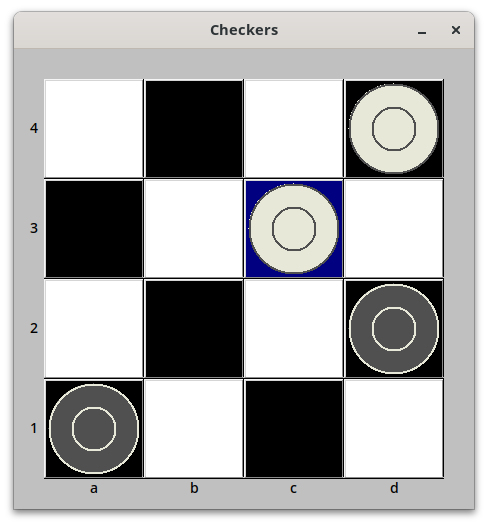
\includegraphics[width=0.5\textwidth]{images/checkers.png}

    }
    \caption{Шахматная доска \(4\times 4\) с~шашками}
    \label{fig:checkers}
\end{figure}

\todo{Описание будет добавлено позже.}



%%================
\WhatToReadSection
%%================
\textcite{Stroustrup:2016:ru}: \textbf{глава~17}



%%===============
\ExercisesSection
%%===============
\begin{exercise}
\item Выполните упражнения из~\textbookref{главы~16} учебника.

\end{exercise}
